\documentclass[../main.tex]{subfiles}

\begin{document}
In this chapter, the implementation details of the approach outlined in Chapter \ref{sec:SolutionArchitecture} will be discussed. Starting from the modelling of the system as a MDP, the implementation of the reinforcement learning algorithm, the disturbance estimation with GP regression, and finally the safe set calculation with HJI reachability analysis will be described.
\section{Markov Decision Process Model}\label{sec:implementation_MDP}
Consider a damped inverted pendulum system with mass $m$, length $l$ and friction coefficient $b$. The states of the system are the pendulum angle $x_1$ and angular velocity $x_2$. The system is disturbed by an additive state-dependent disturbance $d(x)$. The dynamics are described by \cite{doya2000reinforcement}:
\begin{align}
    \dot{x_1} &= x_2\\
    \dot{x_2} &= \frac{1}{ml^2}u+\frac{g}{l}\sin(x_1)-\frac{b}{m}x_2+d(x).
\end{align}
All constants are assumed to be positive. 
Modelling the inverted pendulum system as a MDP means to define the quintuple $(S,A,T,r,\gamma)$ as given in Section \ref{sec:RL}. Defining the finite set of states $S$ and the finite set of actions $A$ implies discretisation over the intervals $[x_{\min}, x_{\max}]$ and $[u_{\min}, u_{\max}]$, where $x_1$ is a circular state and should be wrapped if the discretisation interval is larger than its period $2\pi$. The number of discretisation  steps impacts the convergence speed of the reinforcement learning algorithm and was chosen around $n = 19$ for each state dimension so that we end up with 361 states in total.
The transition probabilities $T$ have been approximated by simply sampling the discrete transitions under a chosen time step $h$. Given a specific action and state, the subsequent state has been simulated $100$ times. The probability $p(s'|s,a)$ of state $s'$ is then computed as the number of transitions to $s'$ from the chosen state and action divided by the number of total transitions. It is hereby important that the time step $h$ is large enough to actually allow transitions. If $h$ is too small, the system will always stay in state $s$ regardless of the chosen action. For the present system, a time step around $h = 0.2\,\text{s}$ has proven to give good results. The reward function for state $s$, $r(s)$, is defined as
\begin{equation}
    r(s) = e^{-\frac{\|s\|^2}{\sigma^2}},
\end{equation}
where $\sigma$ is a constant defining how narrow the function is. Defining the coordinate system with $x_1 = 0$ being on the top, this reward corresponds to the goal of keeping the pendulum still and upright as the states with the smallest $x$ are rewarded the most. The discount factor $\gamma$ is chosen to be $0.9$. This choice weighs future rewards slightly less than present rewards. A possible interpretation of the discount factor is to assume that the agent only has a limited life span. If $\gamma$ is the probability to survive at time step $t$, the life span of the agent will be $\frac{1}{1-\gamma}$. Knowing the life span of the agent, one could then choose the discount factor accordingly. The learning agent in the present system does indeed have a limited life span, because the pendulum is being reset as soon as the state values are outside some margin around the border of the MDP. This is done as part of the algorithm, because learning can only take place inside the MDP. However, it is hard to determine what the expected life span of the present agent is. Our choice of $\gamma = 0.9$ is rather justified by the fact that the convergence time rapidly increases as the discount factor approaches 1. 

\section{Reinforcement Learning}
To our learning agent (the inverted pendulum controller), the reward and transition probabilities are not known beforehand. The agent acts in an unknown environment and aims at maximising an external reward. We therefore apply reinforcement learning to learn the optimal policy. 

\newtheorem{theorem}{Theorem}
\newtheorem{definition}{Definition}
\newtheorem{lemma}{Lemma}
\newtheorem{proposition}{Proposition}
\newtheorem{corollary}{Corollary}
\newtheorem{remark}{Remark}
\def\NoNumber#1{{\def\alglinenumber##1{}\State #1}\addtocounter{ALG@line}{-1}}
\def\hpi{\widehat{\pi}}
\def\hphi{\widehat{\phi}}
\def\M{{\mathbb M}}
\def\NN{{\mathbb N}}
\def\EE{{\mathbb E}}
\def\PP{{\mathbb P}}
\def\RR{{\mathbb R}}
\def\ind{{\mathbf{1}}}
\def\ore{\overrightarrow{e}}
\def\orE{\overrightarrow{E}}
\def\ole{\overleftarrow{e}}
\def\d{\partial}
\def\bx{\bold{x}}
\def\bw{\bold{w}}
\def\bB{\bold{B}}
\def\balpha{\bold{\alpha}}
\def\Poi{\text{Poi}}
\def\Bin{\text{Bin}}
\def\odeg{\overline{\text{deg}}}
\def\Acal{{\mathcal A}}
\def\Pcal{{\mathcal P}}
\def\Ocal{{\mathcal O}}
\def\Rcal{{\mathcal R}}
\def\Scal{{\mathcal S}}
\def\Dcal{{\mathcal D}}
\def\Qcal{{\mathcal Q}}
\def\Bcal{{\mathcal B}}
\def\Ical{{\mathcal I}}
\def\Hcal{{\mathcal H}}
\def\Ncal{{\mathcal N}}
\def\Mcal{{\mathcal M}}
\def\Lcal{{\mathcal L}}
\def\Gcal{{\mathcal G}}
\def\Xcal{{\mathcal X}}
\def\Ucal{{\mathcal U}}
\def\Vcal{{\mathcal V}}
\def\Zcal{{\mathcal Z}}
\def\BUT{{\mathcal{BUGWT}}}
\def\cGr{{{\mathcal G}_d}}
\def\Yb{\bold{Y}}
\def\bY{\bold{Y}}
\def\bI{\bold{I}}
\def\bZ{\bold{Z}}
\def\bW{\bold{W}}
\def\bM{\bold{M}}
\def\Xb{\bold{X}}
\def\bX{\bold{X}}
\def\omu{\overline{\mu}}
\def\oq{\overline{q}}
\def\bac{\backslash}
\def\kl{\mathrm{KL}}
\def\klber{\mathrm{kl}}
\def\supp{\mathrm{supp}}
\def\indic{\mathbbmss 1}
\def\alsp{\vspace{1mm}} 

\def\PF{\mathsf{pf}}
\def\algoM{\textsc{FairBand}}

\newcommand{\sk}{\nonumber\\}

\newcommand{\iskip}{{\vskip -0.4cm}}
\newcommand{\siskip}{{\vskip -0.2cm}}

\newcommand{\bp}{\noindent{\emph{Proof}.}\ }
\newcommand{\ep}{\hfill $\Box$}

\newcommand{\BEAS}{\begin{eqnarray*}}
\newcommand{\EEAS}{\end{eqnarray*}}
\newcommand{\BEA}{\begin{eqnarray}}
\newcommand{\EEA}{\end{eqnarray}}
\newcommand{\BEQ}{\begin{equation}}
\newcommand{\EEQ}{\end{equation}}
\newcommand{\BIT}{\begin{itemize}}
\newcommand{\EIT}{\end{itemize}}
\newcommand{\BNUM}{\begin{enumerate}}
\newcommand{\ENUM}{\end{enumerate}}
\newcommand{\argmin}{\arg\!\min}
\newcommand{\argmax}{\arg\!\max}

\renewcommand{\algorithmiccomment}[1]{\hfill\eqparbox{COMMENT}{// #1}}

\begin{algorithm}[h!]
\small
   \caption{\textsc{Modification of Delayed Q-Learning}}
   \label{alg:alg1}
\begin{algorithmic}
   \REQUIRE $\Scal, \Acal,\gamma$, and $R_{\max}$, $m_0$, $\varepsilon_{\mathrm{target}}$. 
   \FORALL{$(s,a)$}
    \STATE $Q(s, a) \leftarrow R_{\max}/(1-\gamma)$ {\color{blue}  \COMMENT{\texttt{optimistic initialization of $Q$-values}}} 
    \STATE $U(s,a) \leftarrow 0$    {\color{blue} \COMMENT{\texttt{per-batch cumulative $Q$-values for $(s,a)$}}}
    \STATE $B(s, a) \leftarrow 0$   {\color{blue}  \COMMENT{\texttt{beginning time-step of attempted update for $(s,a)$}}}
    \STATE $C(s,a) \leftarrow 0$    {\color{blue}  \COMMENT{\texttt{per-batch counter for $(s,a)$}}} 
    \STATE $M(s, a) \leftarrow m_0$          {\color{blue}  \COMMENT{\texttt{batch size for $(s,a)$}}}  
    \STATE $L(s,a)\leftarrow \textsf{TRUE} $   {\color{blue} \COMMENT{\texttt{the learning flag}}} 
   \ENDFOR
   \STATE $t_{\textrm{update}} \leftarrow 0$  {\color{blue}  \COMMENT{\texttt{time-step of the most recent $Q$-value change}}}
   \STATE $\varepsilon \leftarrow 10^{-4}$    {\color{blue}  \COMMENT{\texttt{threshold for admitting $Q$-value updates}}}
   
   \FOR{$t\geq 1$}   %\qquad\qquad\qquad\qquad {\color{blue}  {\texttt{// main loop}}}
    \STATE Observe the current state $s_t$. Take action $a_t \in \argmax_{a\in \Acal} Q(s_t, a)$, receive reward $r_t$, and go to a next state $s_{t+1}$.    \alsp
    \IF{$B(s_t,a_t)\le t_{\textrm{update}}$} \alsp
        \STATE $L(s_t,a_t) \leftarrow \textsf{TRUE}$ \alsp
    \ENDIF
    
    \IF{$L(s_t,a_t)$=\textsf{TRUE}} \alsp
        \IF{$C(s_t,a_t)=0$} \alsp
            \STATE $B(s_t,a_t)\leftarrow t$ \alsp
        \ENDIF
        \STATE $C(s_t,a_t) \leftarrow C(s_t,a_t) + 1$ \alsp
        \STATE $U(s_t, a_t) \leftarrow U(s_t, a_t) + r_t + \gamma \max_{a\in \Acal} Q(s_{t+1}, a)$   \alsp
        \IF{$C(s_t,a_t)=M(s_t,a_t)$} \alsp
            \STATE $q \leftarrow U(s_t, a_t)/M(s_t,a_t)$ \alsp
            \IF{$|Q(s_t,a_t)-q|\ge \varepsilon$} \alsp
                \STATE $Q(s_t,a_t) \leftarrow q$ \alsp  {\color{blue}  \COMMENT{\texttt{update if $Q$-value changes significantly }}}
                \STATE $t_{\textrm{update}} \leftarrow t$ \alsp
            \ELSIF{$B(s_t,a_t)>t_{\textrm{update}}$} \alsp
                \STATE $L(s_t,a_t) \leftarrow \textsf{FALSE}$ \alsp
            \ENDIF
            \STATE $U(s_t,a_t) \leftarrow 0$ \alsp
            \STATE $C(s_t, a_t) \leftarrow 0$ \alsp
            \STATE $M(s_t, a_t) \leftarrow \min\{\lceil 1.02M(s_t,a_t)\rceil +1, 500\}$  {\color{blue} \alsp //{\texttt{increase batch size}}}
            \STATE $\varepsilon \leftarrow \min \{1.1\varepsilon, \varepsilon_{\mathrm{target}}\}$   {\color{blue}  \COMMENT{\texttt{increase the threshold}}}
        \ENDIF
    \ENDIF
   \ENDFOR             

\end{algorithmic}
\end{algorithm}


The chosen algorithm, introduced in \cite{talebi2017modified}, resembles largely the Delayed Q-Learning algorithm introduced in Section \ref{sec:RL} with the update rule \eqref{DelayedQ}. The only difference lies in the handling of the algorithm inputs $\varepsilon$ and $m$. The batch size $m$ determines how often the update of a state-action pair's Q-value is attempted until a successful update of any Q-value has to occur for the update to be attempted again. This batch size has been replaced by the state-action-dependent batch size $M(s,a)$ that is increased each time when the update of the state-action pair $(s,a)$ has been tried $M(s,a)$ times. More specifically, the update rule is 
\begin{align}
    M_{t+1}(s_t,a_t) &= \min\{\lceil1.02M_t(s_t,a_t)\rceil+1, 500\}\\
    M_{t+1}(s,a) &= M_t(s,a), \qquad \forall (s,a) \neq (s_t,a_t).
\end{align}
The threshold $\varepsilon$ for an update to be admitted has been made adaptive such that $\varepsilon$ after $M(s,a)$ attempted updates increases to 
\begin{equation}
    \varepsilon_{t+1} = \min\{1.1 \varepsilon_t, \varepsilon_{\text{target}}\}, 
\end{equation}
where $\varepsilon_{\text{target}}$ is an input parameter.
The initialization of the Q-values is done optimistically according to \eqref{eq:optimistic_init}. The learning rate is chosen to be $\alpha(s,a) = \frac{1}{v+1}$ where $v$ is the number of times that the current state-action pair $(s_t,a_t)$ has been visited. This learning rate leads to a faster convergence than $\alpha(s,a) = \frac{1}{t+1}$ with step count $t$ and fulfills still the convergence criterion posed in \eqref{eq:stepsize}. Without any safety-preserving controller, this algorithm converges to the optimal policy but does not guarantee the satisfaction of constraints. Figure \ref{fig:PolicyComparison_unsafe} shows the learned policy after a test run with $100,000$ steps in comparison with the optimal policy that has been found with policy iteration. The colours correspond to certain action values. As the actual values are not of importance, no legend matching colours to values has been provided. It can be seen that the estimated policy is relatively accurate, however the learning algorithm violates the boundaries of the MDP no less than $8986$ times. As the algorithm learns the optimal policy, the number of constraint violations decreases. This can be seen in Figure \ref{fig:Histogram_ConstraintViolations}, where a histogram of the constraint violations is shown. However, safety can never be guaranteed in this framework. To prevent occurrence of these violations, a safe controller will be introduced in the next section.


\begin{figure}[H]
    \centering
    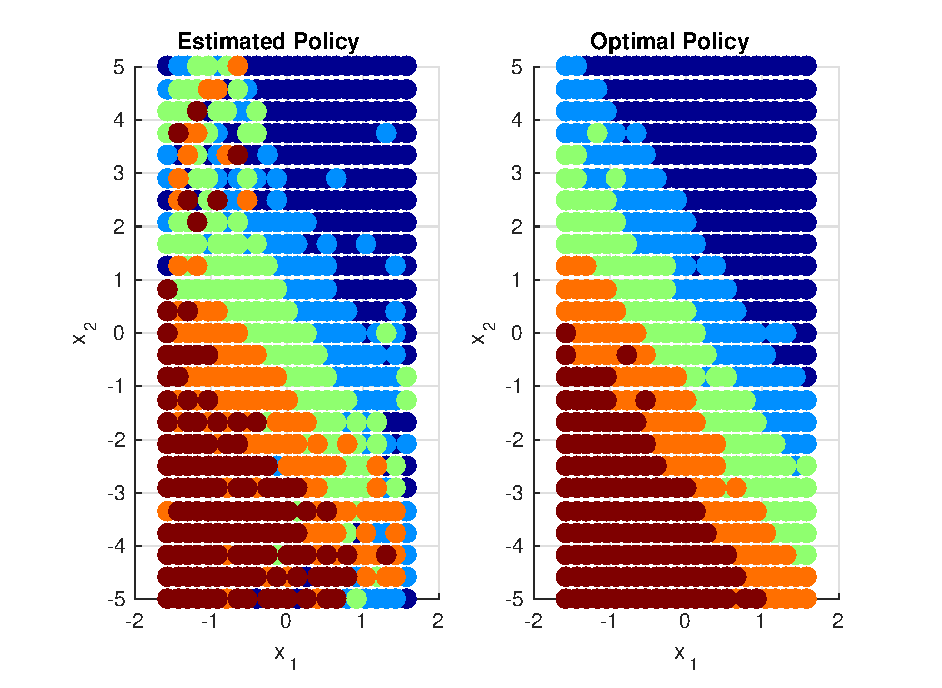
\includegraphics[width=\textwidth]{PolicyComparison_unsafe}
        \caption{The learned policy versus the optimal policy.}    
    \label{fig:PolicyComparison_unsafe}
\end{figure}
\begin{figure}[H]
    \centering
    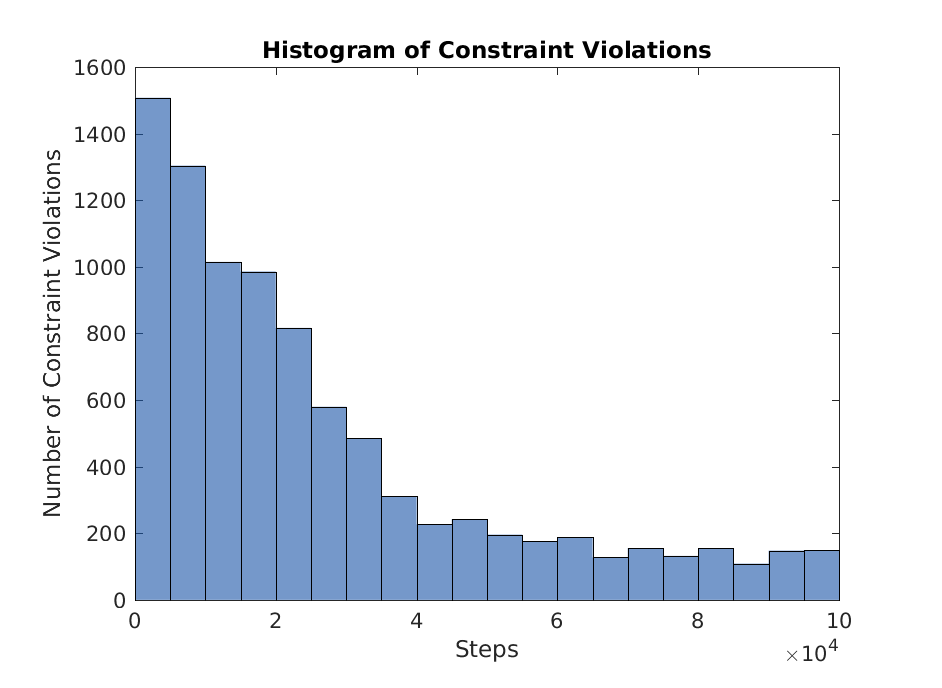
\includegraphics[width=\textwidth]{Histogram_ConstraintViolations}
        \caption{Evolution of the constraint violations with increasing number of steps.}    
    \label{fig:Histogram_ConstraintViolations}
\end{figure}

\section{Safe Set Computations based on Reachability Analysis}
The general idea behind safe set computations has been described in Section \ref{sec:SafeSets}. In this section, the concrete implementation of such computations for the case of the inverted pendulum system will be described. The Hamiltonian in this case becomes 
\begin{equation}\label{eq:hamil_implementation}
    H(x,p) = \max_{u \in \mathcal{U}} \min_{d \in \mathcal{D}} p^T 
\left(
\begin{array}{c}
x_2\\
\frac{1}{ml^2}u+\frac{g}{l}\sin(x_1)-\frac{b}{m}x_2+d\\
\end{array}
\right).
\end{equation}
Determining the optimizers to \eqref{eq:hamil_implementation} can be done easily for non-linear systems whose inputs enter linearly. That means that the dynamics can be written on the form
\begin{equation}
    f(x,u,d) = f_1(x)+\textbf{F}_2(x)u+\textbf{F}_3(x)d.
\end{equation}
This is the case for the inverted pendulum system with
\begin{align}
    f_1(x) &= \left(
\begin{array}{c}
x_2\\
\frac{g}{l}\sin(x_1)-\frac{b}{m}x_2\\
\end{array}
\right),\\
    \textbf{F}_2(x) &= \left(
\begin{array}{c}
0\\
\frac{1}{ml^2}\\
\end{array}
\right),\\
    \textbf{F}_3(x) &= \left(
    \begin{array}{c}
0\\
1\\
\end{array}
\right).
\end{align}
According to \cite{mitchell2004toolbox}, the input maximising \eqref{eq:hamil_implementation} and the disturbance minimising the equation are then given by 
\begin{align}
    u^*(x,p)&=
\begin{cases}
  \underline{U},\qquad \text{if } \sum_{j=1}^n p_j \textbf{F}_{2,j}(x)\leq 0;\\
  \overline{U}, \qquad \text{otherwise,}
\end{cases}\\
    d^*(x,p)&=
\begin{cases}
  \overline{D},\qquad \text{if } \sum_{j=1}^n p_j \textbf{F}_{3,j}(x)\leq 0;\\
  \underline{D}, \qquad \text{otherwise}.
\end{cases}
\end{align}
Hence, $\overline{U}$ and $\underline{U}$ describe the input constraints $u\in \mathcal{U} = [\underline{U},\overline{U}]$. Moreover $\overline{D}$ and $\underline{D}$ constitute the disturbance range $d\in \mathcal{D} = [\underline{D},\overline{D}]$. 

\iffalse

By defining 
\begin{align}
    U_{\text{max}} &= \max(|\underline{U}|,|\overline{U}|), \\
    D_{\text{max}} &= \max(|\underline{D}|,|\overline{D}|), 
\end{align} 
$u^*$ and $d^*$ can be explicitly written as
\begin{align}
    u^*(x,p) &= \frac{U_{\text{max}}}{ml^2} \cdot \text{sign}(p_2)\\
    d^* &= -D_{\text{max}} \cdot \text{sign}(p_2).
\end{align}

\begin{equation}\label{eq:hamil_explicit}
    H(x,p) = p_1x_2+p_2\left(\frac{g}{l}\sin(x_1)-\frac{b}{m}x_2\right)+|p_2|\left(\frac{1}{ml^2}U_{\text{max}}-D_{\text{max}}\right).
\end{equation}
\fi
Hence, the Hamiltonian can be written as
\begin{equation}\label{eq:hamil_explicit}
    H(x,p) = p_1x_2+p_2\left(\frac{g}{l}\sin(x_1)-\frac{b}{m}x_2+\frac{1}{ml^2}u^*(x,p)+d^*(x,p)\right).
\end{equation}
$H(x,p)$ as given above must be coded into an existing function prototype within the toolbox.
To calculate the derivative $p = \frac{\partial}{\partial x} \phi(x,t)$, the Level Set toolbox employs the Lax-Friedrichs approximation 
\begin{equation}
    \widehat{H}(x,p^+,p^-) \overset{\Delta}{=} H\left(x,\frac{p^-+p^+}{2}\right) - \frac{1}{2} \alpha^T(x)(p^+-p^-)
\end{equation}
where $p^+$ and $p^-$ are respectively left and right side approximations of $p$, and where $H(x,p)$ is given in \eqref{eq:hamil_explicit}. The function $\alpha(x)$ must also be implemented within the provided function prototype. $\alpha(x)$ is given to be
\begin{equation}
    \alpha_i(x) = \max_{p\in\mathcal{I}} \left|\frac{\partial H}{\partial p_i}\right|,
\end{equation}
with $\mathcal{I}$ being the hypercube containing all values that $p$ takes over the computational domain. The calculation can be done with the following over-approximation
\begin{equation}
    \alpha_j(x) \leq |f_j^x(x)| + |\textbf{F}_{2,j}|U_{\text{max}} + |\textbf{F}_{3,j}|D_{\text{max}}, 
\end{equation}
which for the present system reduces to 
\begin{align}
    \alpha_1 &\leq |x_2|,\\
    \alpha_2 &\leq \left|\frac{g}{l}\sin(x_1)-\frac{b}{m}x_2\right| + \frac{1}{ml^2}U_{\text{max}} + D_{\text{max}}.
\end{align}
Having specified the functions for calculating $H(x,p)$ and $\alpha(x)$, the Level Set toolbox can be adapted for the present problem. Specifically, a function has been written that takes as inputs an estimate for the disturbance bounds $\underline{D}$ and $\overline{D}$, input constraints $\underline{U}$ and $\overline{U}$, an initial safe set $\mathcal{S}_0$, a time horizon $\tau$, and the state-space of the MDP. For each state in the MDP, the function outputs, whether it is safe under time horizon $\tau$ and a safe control $u^*(s)$. During the learning process, one can then apply the safe control as soon as the system hits the border of the safe set. To illustrate this, Figure \ref{fig:safeSet_example} shows the evolution of a safe set calculation over the time horizon $\tau = 30\,\text{s}$. The first subplot shows the initial safe set $\mathcal{S}_0$ as defined by the function input. Over time, the safe set is shrinking to the set $\mathcal{S}_\tau$ shown in the last subplot. Trajectories starting from within this set are guaranteed to remain in $\mathcal{S}_0$ for $t = [0, \tau]$. It can easily be seen that the set converges already within the first seconds such that trajectories that are safe for $t = [0, 10]$ are also safe for the whole time horizon. 

\begin{figure}[H]
    \centering
    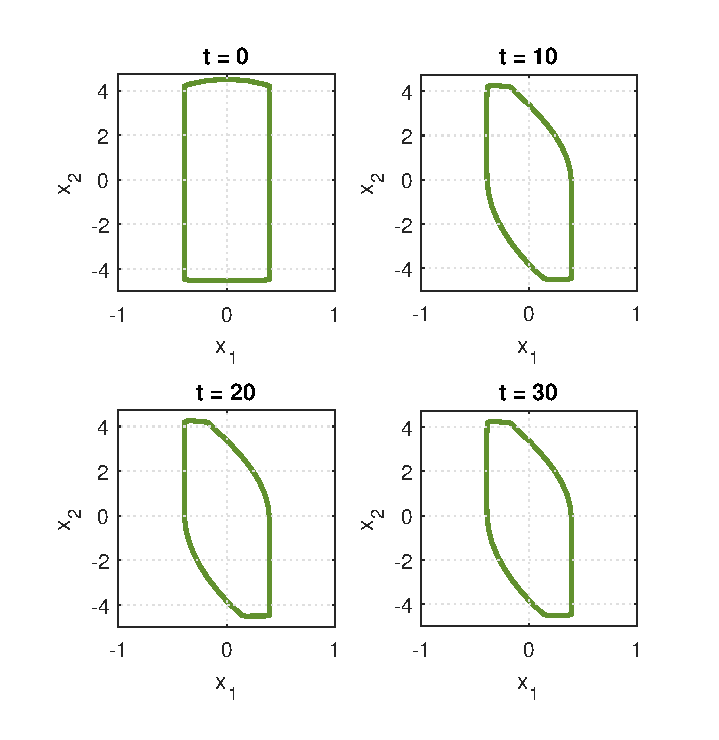
\includegraphics[width=\textwidth]{safeSet_example}
        \caption{Example for the evolution of a safe set during the time horizon.}    
    \label{fig:safeSet_example}
\end{figure}

To verify the calculations, simulations of system trajectories have been done for both, initial conditions within the safe set $\mathcal{S}_\tau$ and outside that set. The results are depicted in Figure \ref{fig:safeSet_simulation}. Trajectories are marked with a red dot at the initial condition and a blue dot at the final value. The safety-preserving controller manages to keep all trajectories with initial conditions inside $\mathcal{S}_\tau$ within the safe set for the whole simulation time. The simulation time has been chosen to be smaller than the time horizon $\tau = 30 \,\text{s}$ to keep the computation time short and the figure clean. The result holds however for longer simulation times. Furthermore, the figure indicates that the safe set is an under-approximation of the true safe set as the trajectories with initial conditions close to $\mathcal{S}_\tau$ can be stabilized too. This is expected as the calculated reachable set is an over-approximation of the true reachable set. \par
\begin{figure}[h]
    \centering
    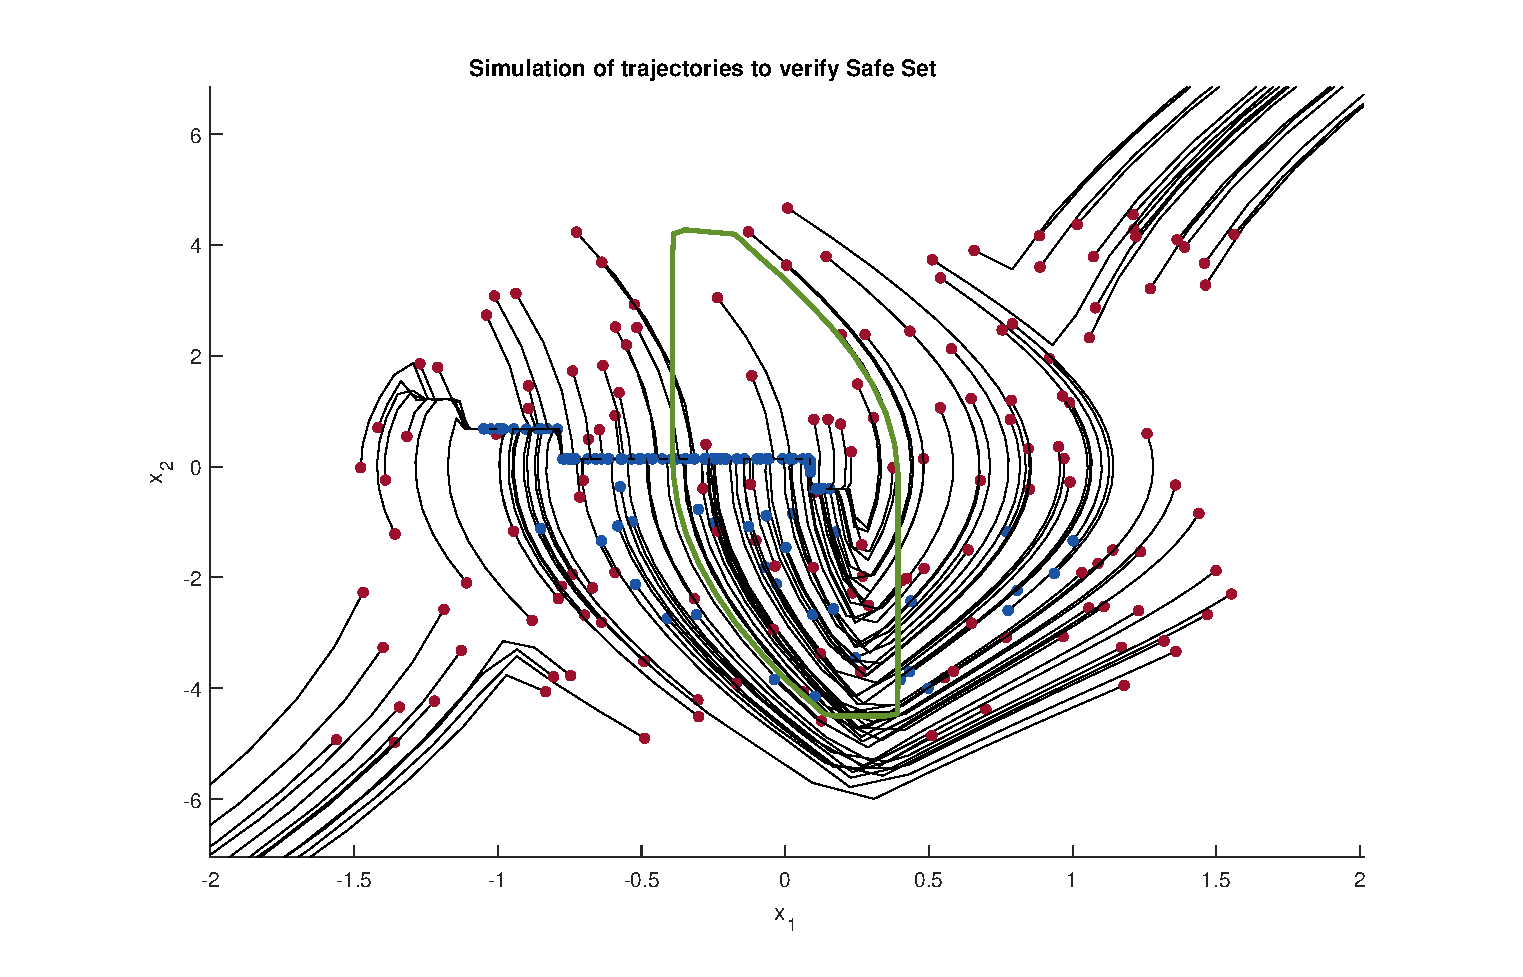
\includegraphics[width=\textwidth]{safeSet_simulation}
        \caption{Simulations to verify the control invariance of the safe set.}    
    \label{fig:safeSet_simulation}
\end{figure}
It is worth mentioning that the safe set calculations assume continuous dynamics. It is therefore important to keep the time step $h$ small enough so that the discretisation error does not become too large. This conflicts with the requirement of Section \ref{sec:implementation_MDP}, which necessitates the time step to be large in order to allow transitions between states. With a very small time step learning can not take place as no state transitions can be made. On the other hand, a large time step jeopardises safety as the system possibly violates the border of the safe set between two samples and it is then not guaranteed that the safe control can bring the system back into the borders again. Ideally, one would find a systematic way to shrink the safe set dependent on the time step in order to account for the error caused by discretisation. This falls beyond the scope of this thesis. \par 
The problem is tackled otherwise by introducing a ``safety loop" that runs faster than the actual learning loop. For instance, if the time step required from the MDP is $h_{\text{learn}} = 0.12\,\text{s}$, but the time step for the safety-preserving controller should be maximal $h_{\text{safe}} = 0.02\,\text{s}$, the safety loop will run six times faster than the learning loop. In each safety iteration the evolution of the system is simulated. If the system violates the boundaries of the safe set, the safe control is applied. Otherwise the learning control (that is constant over the six safety iterations) is applied. This is portrayed in Figure \ref{fig:doubleloop}. During the fourth iteration, the safe controller detects a violation of the safe set boundaries and applies the safe control that brings the system back inside the boundaries. For the sake of illustration, the time steps are chosen very large in comparison to the drawn safe set. Obviously, one would not choose the time step $h_{\text{learn}}$ so large that the whole safe set can be crossed within one time step.

\begin{figure}[H]
    \centering
    \begin{subfigure}[t]{0.45\textwidth}
        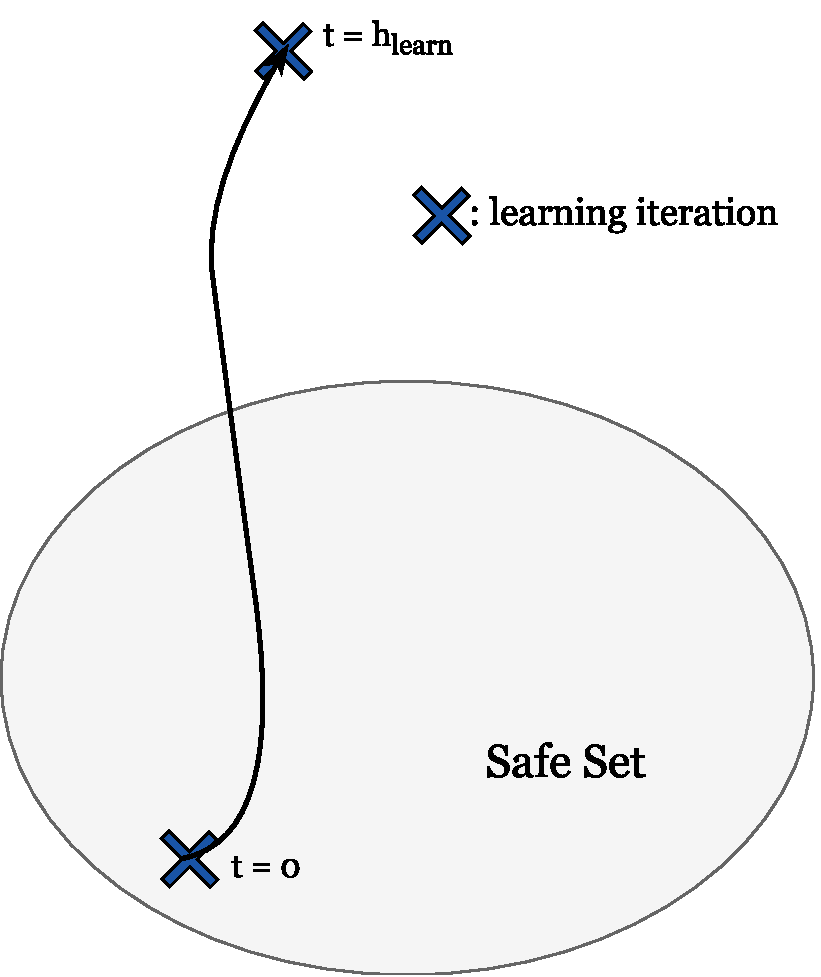
\includegraphics[width=\textwidth]{doubleloop_fail}
    \end{subfigure}%
    ~ 
    \begin{subfigure}[t]{0.55\textwidth}
        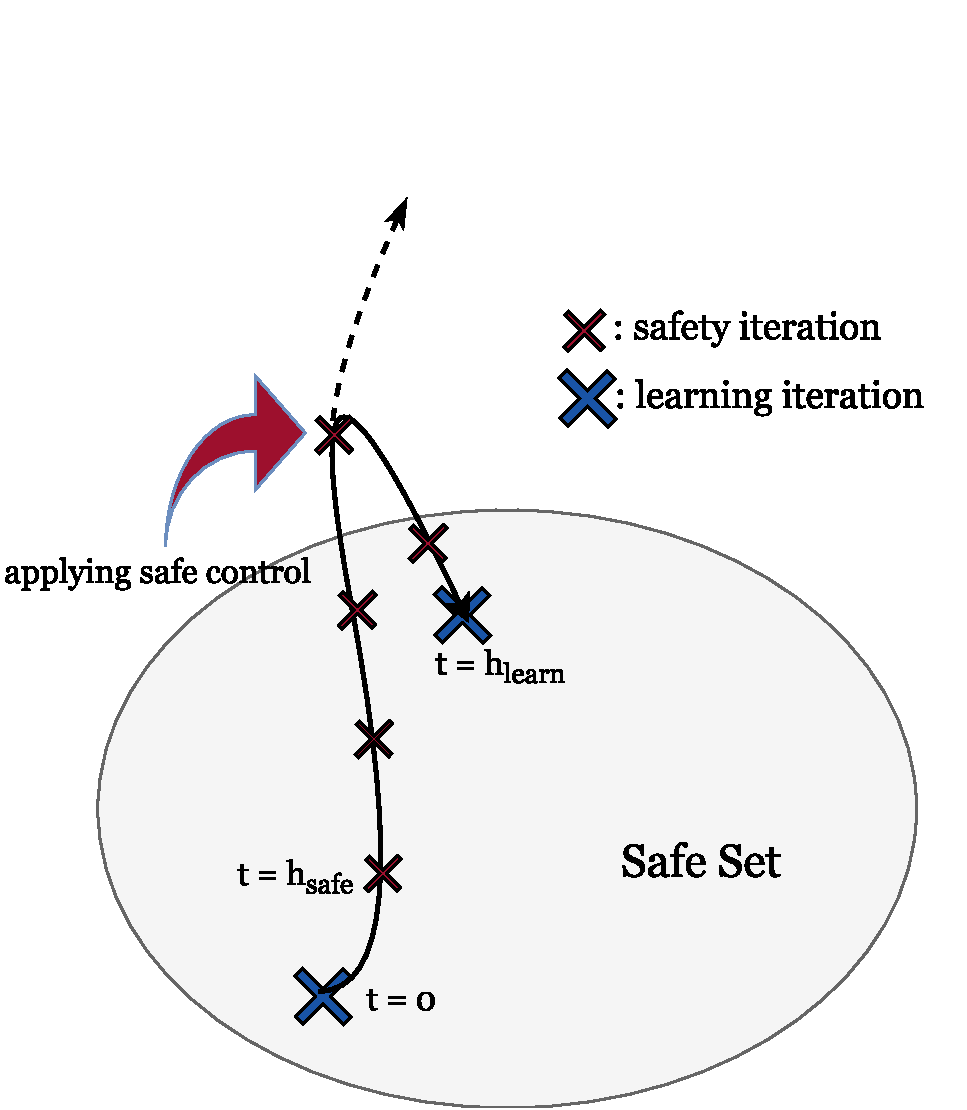
\includegraphics[width=\textwidth]{doubleloop}
        \end{subfigure}
        \caption{Illustration of the problem with a large time step $h_{\text{learn}}$. At $t= h_{\text{learn}}$ the system is without safety check (left) already far outside the safe set so that it cannot be guaranteed to be brought back again. On the right hand side, the same example is shown with a faster running safety loop. Each $h_{\text{safe}}$ a safety check is performed so that the violation of the safe set can be detected and acted against earlier.}\label{fig:doubleloop}  
\end{figure}

\section{Disturbance Estimation with Gaussian processes}\label{sec:implementation_GP}
In this section, the disturbance estimation with GP regression will be described. As stated above, the safe set calculations with HJI reachability analysis rely on a given bound for the disturbance. This bound is initially picked in a conservative manner but should be updated as soon as data from the real system is available. Given some measurements of the state $x$ collected during the learning process, disturbance samples can be obtained by calculating:
\begin{equation}
    \hat{d}(x)=\dot{x}_2-\left(\frac{1}{ml^2}u+\frac{g}{l}\sin(x_1)-\frac{b}{m}x_2\right).
\end{equation}
As the continuous derivative $\dot{x}_2$ is not available, an approximation with the forward difference is calculated:
\begin{equation}
    \dot{x}_2 \approx \frac{x_{2,k+1}-x_{2,k}}{h},
\end{equation}
where $x_{2,k+1}$ and $x_{2,k}$ are two consecutive samples and $h$ is the sample time.
For this approximation to be accurate, it is important that the time step $h$ is small enough. Therefore, the samples are recorded within the faster running safety loop, so that $h$ from the above equation is given as $h = h_{\text{safe}}$.
In order to obtain estimates for $d$ for all values of $x$ and not only for the sampled values, a GP model is employed. GPs have the advantage to provide not only an estimate, but also the standard deviation that serves as a measure of uncertainty. Hence, we can pick the range of $d(x)$ to be
\begin{align}
    \underline{d}(x) &= \mu(x)-3\sigma(x)\\
    \overline{d}(x) &= \mu(x)+3\sigma(x).
\end{align}
Here, $\mu(x)$ is the mean of the estimate and $\sigma(x)$ is its standard deviation. The chosen  probabilistic bounds for $\overline{d}$ and $\underline{d}$ give a confidence interval of $99.7\%$. However, one should be advised that that the numerical differentiation introduces an error that is not accounted for in this confidence interval. This did not pose any problem in the algorithm, because $h_{\text{safe}}$ has been picked sufficiently small to ensure safety. Nevertheless, it might be interesting to account for the error due to numerical differentiation and discrete state-space in a more systematic way when calculating the safe set. \par
Another important question is how to choose sample points that can be fed to the GP regression. As the regression is computationally expensive, it is not possible to feed all recorded samples into the GP. One should rather choose around $1000$ points that accurately and efficiently represent the whole state-space. The question then is how to ensure that the sample points are evenly spread over the whole state-space, so that a good estimate over the whole state-space can be obtained. To achieve this, it is not enough to randomly pick samples because the samples will concentrate around the equilibrium point as soon as a good control is learned. Instead, a set of randomly chosen points that cover the whole state-space is used as a grid. The samples from the system that lie closest to those points are chosen so that it can be ensured that the points around the equilibrium are not over-represented.  This procedure is illustrated in Figure \ref{fig:pointchoice}. One should notice that this is a rather complicated and artificial way of achieving a good spread of the samples. Instead of cherry picking the samples, one should rather encourage the system to actually explore the edges of the safe set. This issue has been dealt with in Section \ref{sec:Exploration}. Furthermore, all chosen samples still will lie within the safe set, as the system is required to never leave this set. However, by getting a less conservative disturbance estimate at the borders of the safe set, it is possible to subsequently enlarge the safe set and therefore the region where samples can be collected.

\begin{figure}
    \centering
    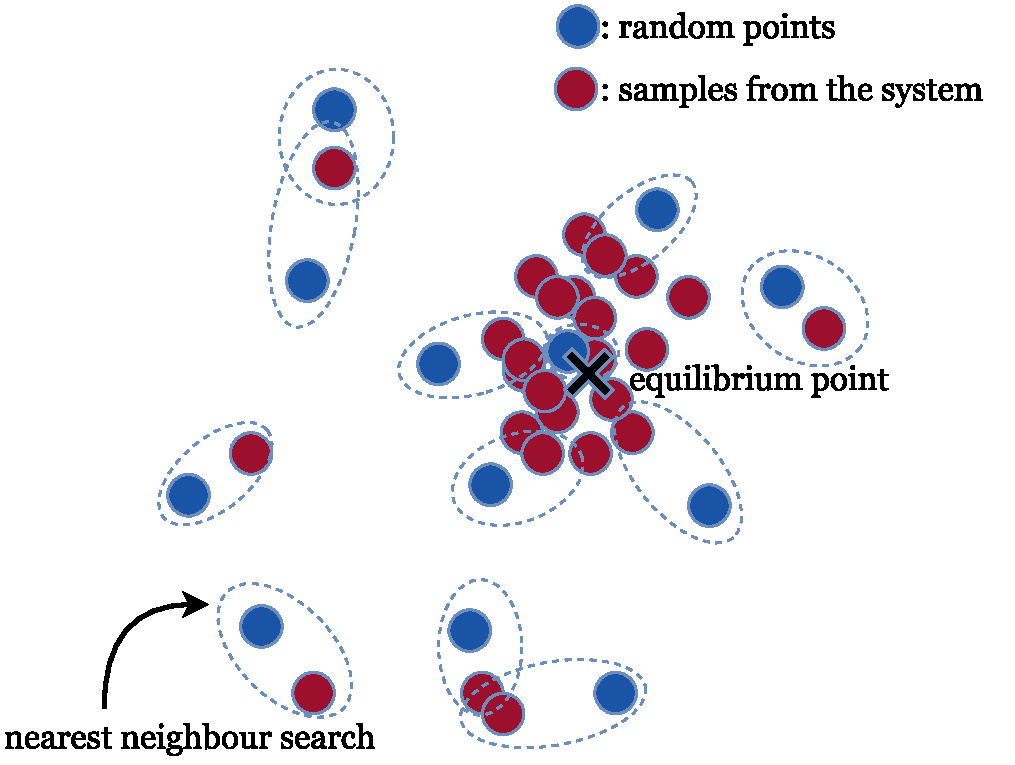
\includegraphics[width=0.8\textwidth]{pointchoice}
        \caption{Choice of samples (red) by employing a grid (blue) and taking the nearest neighbours to the grid points in order to ensure that the samples cover the whole state-space.}  \label{fig:pointchoice}
\end{figure}

We then have a set of evenly spread disturbance samples that can be used for GP regression. The regression is done with the GPML toolbox \cite{Rasmussen:2010:GPM:1756006.1953029} with a zero mean function and a squared exponential kernel as given in \eqref{eq:sqexp}.

Figure \ref{fig:GP_posterior} aims at illustrating the results from a GP regression for a constant disturbance $d = 2 \, \text{N}$ after $48,000$ recorded samples of which $1000$ are fed into the GP. The figure shows $1000$ input samples (blue) that are widely spread within the safe set. The upper and lower planes bound the $\pm 3\sigma$ confidence interval that is additionally shaded in grey. The plane ``sandwiched" in the middle between the two outer planes is the mean, i.e. the disturbance estimate that the GP outputs. In the sliced lower plot, it can be seen that the estimate in the region around the origin is very accurate and the uncertainty is low.
\begin{figure}
    \centering
    \begin{subfigure}[t]{\textwidth}
        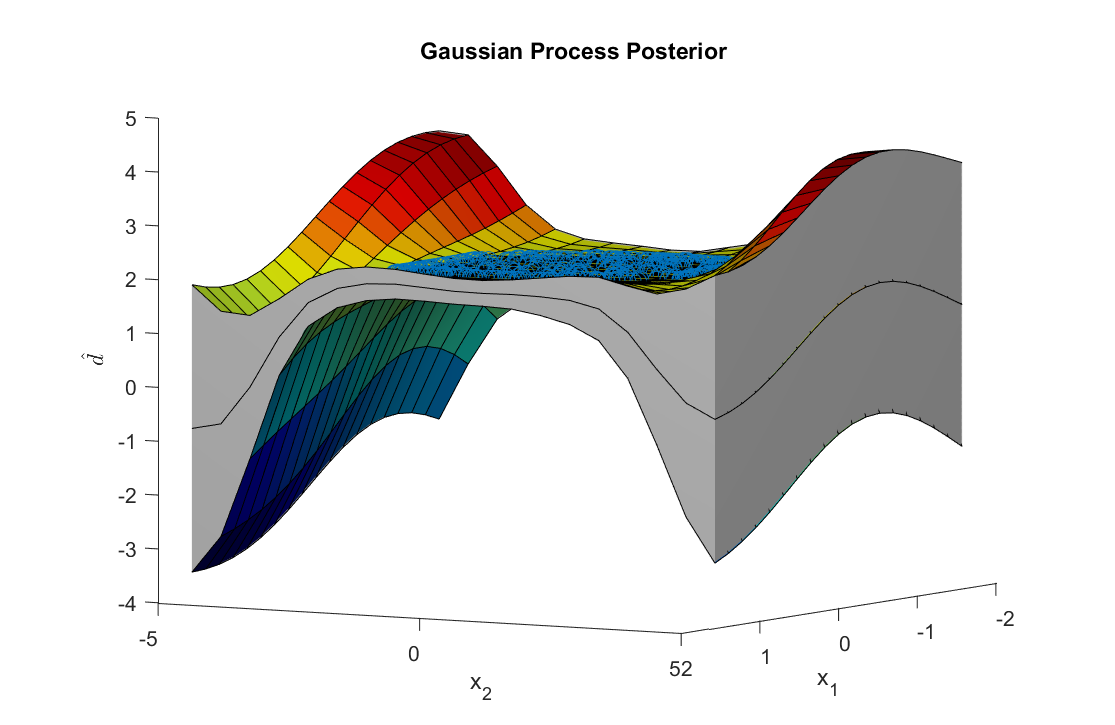
\includegraphics[width=\textwidth]{GP_posterior2}
    \end{subfigure}
    
    \begin{subfigure}[t]{\textwidth}
        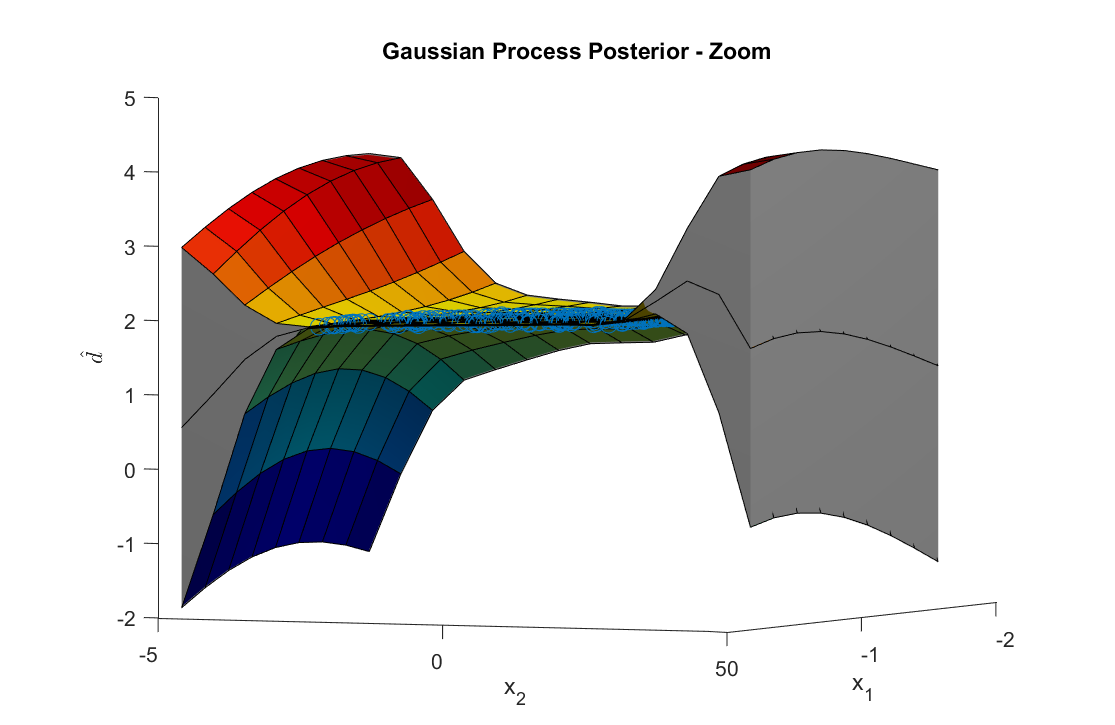
\includegraphics[width=\textwidth]{GP_posterior_zoom}
        \end{subfigure}    \caption{Disturbance estimation with GP regression for a disturbance. The lower and upper planes bound the $\pm 3\sigma$ confidence interval (shaded in grey). The samples that serve as input to the GP are shown as blue circles. The mean plane can be seen as a thin line in the middle of the confidence interval. The lower figure depicts a slice through the middle of the figure to verify the low uncertainty in the middle of the surface.}  \label{fig:GP_posterior}
\end{figure}
\section{Exploration} \label{sec:Exploration}
While this thesis mainly follows the approach presented in \cite{akametalu2014reachability}, this section deals with a topic that has not been treated in that approach: Exploration. Exploration addresses the need of visiting the whole state-space in order to find the optimal strategy instead of only exploiting the one based on readily observed parts of the state-space. In the inverted pendulum system, this corresponds, for instance, to the need for visiting the borders of the safe set in order to get a better disturbance estimate and potentially enlarge the safe set instead of only staying close to the origin. Furthermore, the learning of a control policy for all states requires that all states are visited a sufficient number of times. In Section \ref{sec:implementation_GP}, the need for exploration has been dealt with in a rather unorthodox way. By setting up a grid and doing a nearest neighbour search, it has been ensured that the samples cover the whole state-space. However, this is not exploration, as one does not encourage the system to visit the borders of the safe set, but rather hopes for that the system does so automatically. For this reason, a more essential way of doing exploration will be presented in this section. \par 
The approach chosen is called Incremental Q-learning and modifies the way in which actions are chosen during the learning process. The procedure does not affect the update of the Q-value, so that we still can apply the update rule introduced in Section \ref{sec:implementation_MDP}. Incremental Q-learning aims at a de-randomisation of the $\epsilon$-greedy policy as explained in Section \ref{sec:RL} \cite{even2001convergence}. Instead of choosing random actions with probability $\epsilon$, a greedy policy with respect to the $Q$-values plus a promotion term $A(s,a)$ is chosen. This term promotes state-action pairs that have not been visited often and therefore it encourages exploration. For each state-action pair $(s,a)$, $A(s,a)$ is initialized to zero and updated in the following way:
\begin{equation}
    A_{t+1}(s,a) = 
\begin{cases}
    0,\qquad &\text{if } s_t = s, a_t = a;\\    
    A_{t}(s,a) + \Phi_t(\#(s,a)),\qquad &\text{if } s_t = s, a_t \neq a;\\
    A_{t}(s,a),\qquad &\text{if } s_t \neq s, a_t \neq a.
\end{cases}
\end{equation}
The term $\Phi_t(\#(s,a))$ is the promotion function that depends on the number of times the system visited state $s$ without executing action $a$ since the last time it executed $a$ from $s$. The promotion function chosen in the following is $\Phi_t(i) = \frac{1}{i+1}$. 
\end{document}